\section{Свободное движение}

Рассмотрим систему 2-го порядка, заданную дифференциальным уравнением
\begin{equation}
    \ddot y +a_1\dot y+a_0y=u.
\end{equation}
Сделаем некоторые преобразования для структурной схемы, которую можно
увидеть в рисунке \ref{fig:task_1_slx} (начальные условия задаются в двух
последних интеграторах):
\begin{equation*}
    \begin{array}{c}
        p^2[y]+p[a_1y]+a_0y=u,\\[2mm]
        y=\frac{1}{p^2}[u-a_0y-a_1\dot y].
    \end{array}
\end{equation*}
Для каждого из вариантов задано по шесть наборов значений корней 
характеристического уравнения $\lambda_1$ , $\lambda_2$ и начальных условия 
$y(0), \dot y(0)$. Чтобы вычислить коэффициенты $a_1$ и $a_0$, 
воспользуемся формулами $a_1=-\lambda_1-\lambda_2$, $a_0=\lambda_1\lambda_2$.
Это все можно увидеть в таблице \ref{tab:values}, а аналитические 
решения свободного движения - уравнения со \ref{eq:11} по \ref{eq:16},
вывод которых можно увидеть в конце документа.
Графики моделирования схемы и сравнения с аналитическими решениями можно
увидеть на рисунке \ref{fig:task_1_out}. Все графики (пары моделирования
и аналитического решения) похожи друг на друга. Набор первый и
второй асимптотически устойчивы, третий устойчив по Ляпунову, четвертый, 
пятый и шестой неустойчивы.


\begin{table}[h!]
    \centering
    \begin{tabular}{|c|c|c|c|c|c|c|c|}
    \hline
    \text{№} & $\lambda_1$ & $\lambda_2$ & $y(0)$ & $\dot{y}(0)$ & $a_0$ & $a_1$ \\
    \hline
    1 & $-3$ & $-1.5$ & $1$ & $0$ & $4.5$ & $4.5$ \\
    \hline
    2 & $-1.2 + j10$ & $-1.2 - j10$ & $1$ & $0$ & $101.44$ & $2.4$ \\
    \hline
    3 & $j10$ & $-j10$ & $1$ & $0$ & $100$ & $0$ \\
    \hline
    4 & $1.2 + j10$ & $1.2 - j10$ & $0.05$ & $0$ & $101.44$ & $-2.4$\\
    \hline
    5 & $3$ & $1.5$ & $0.05$ & $0$ & $4.5$ & $-4.5$\\
    \hline
    6 & $-0.8$ & $0.8$ & $0$ & $0.1$ & $-0.64$ & $0$ \\
    \hline
    \end{tabular}
    \caption{\label{tab:values}Таблица корнями характеристического уравнения, начальными условиями и коэффициентами.}
\end{table}

\begin{equation}
    \label{eq:11}
    y_{\text{св}_1}(t)=2e^{-1.5t}-e^{-3t},
\end{equation}
\begin{equation}
    \label{eq:12}
    y_{\text{св}_2}(t)e^{-1.2t}(\cos 10t-0.12\cdot\sin 10t),
\end{equation}
\begin{equation}
    \label{eq:13}
    y_{\text{св}_3}(t)=\cos10t,
\end{equation}
\begin{equation}
    \label{eq:14}
    y_{\text{св}_4}(t)=e^{1.2t}(0.05\cdot\cos10t-0.006\cdot\sin10t),
\end{equation}
\begin{equation}
    \label{eq:15}
    y_{\text{св}_5}(t)=-0.05e^{3t}+0.1e^{1.5t},
\end{equation}
\begin{equation}
    \label{eq:16}
    y_{\text{св}_6}(t)=0.125\cdot\sin0.8t.
\end{equation}

\begin{figure}
    \centering
    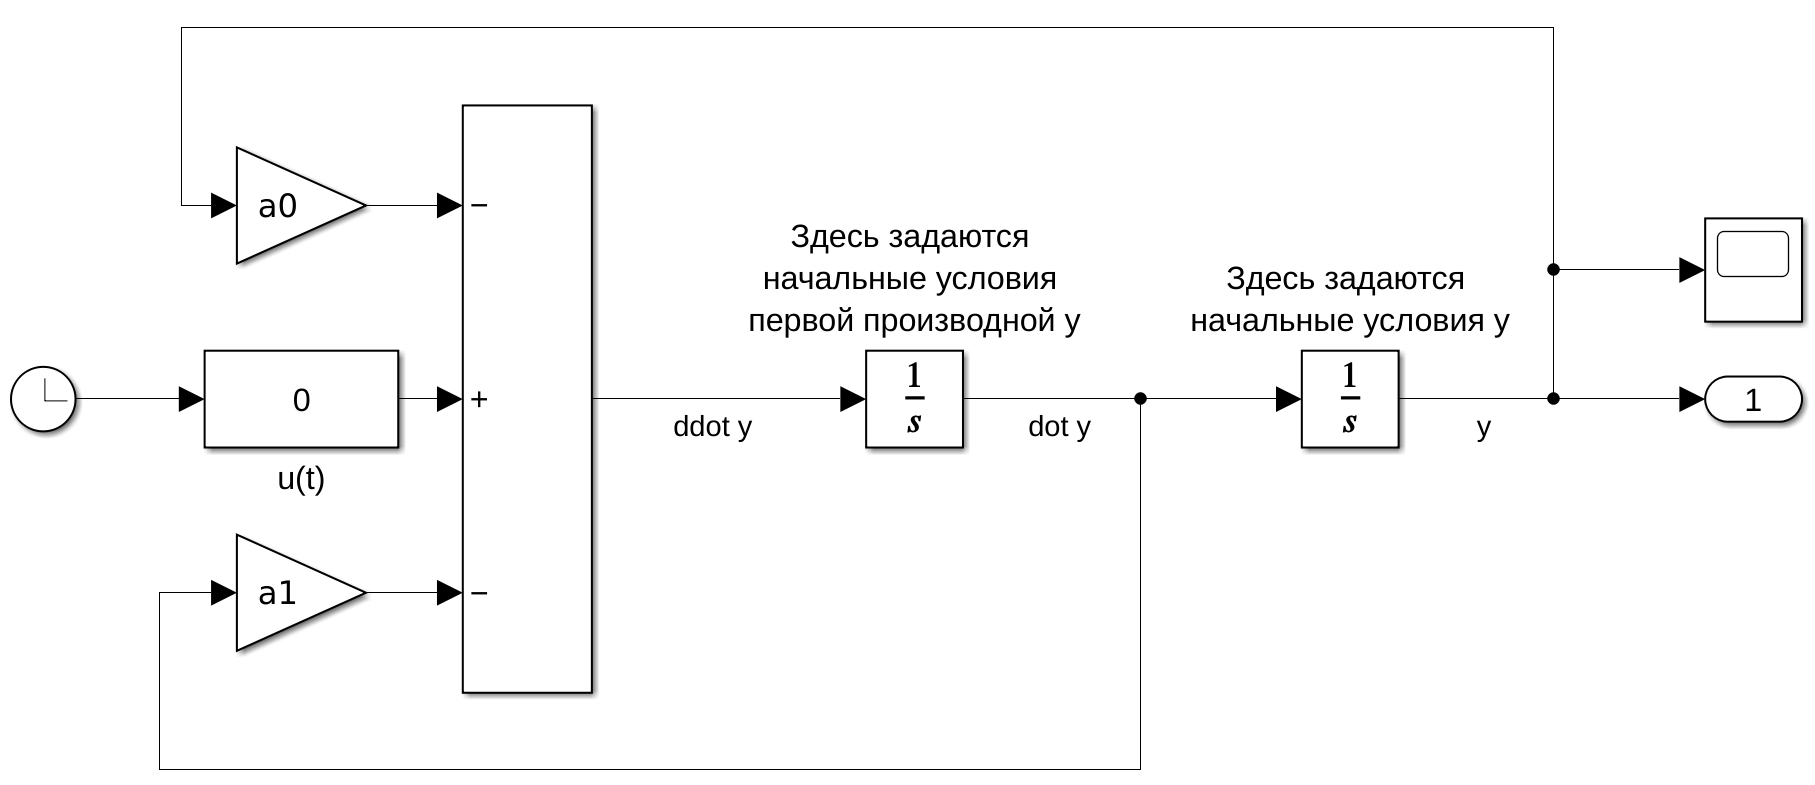
\includegraphics[width=1\textwidth]{figs/task_1_slx.png}
    \caption{Структурная схема дифференциального уравнения задания 1.}
    \label{fig:task_1_slx}
\end{figure}
    
\begin{figure}
    \centering
    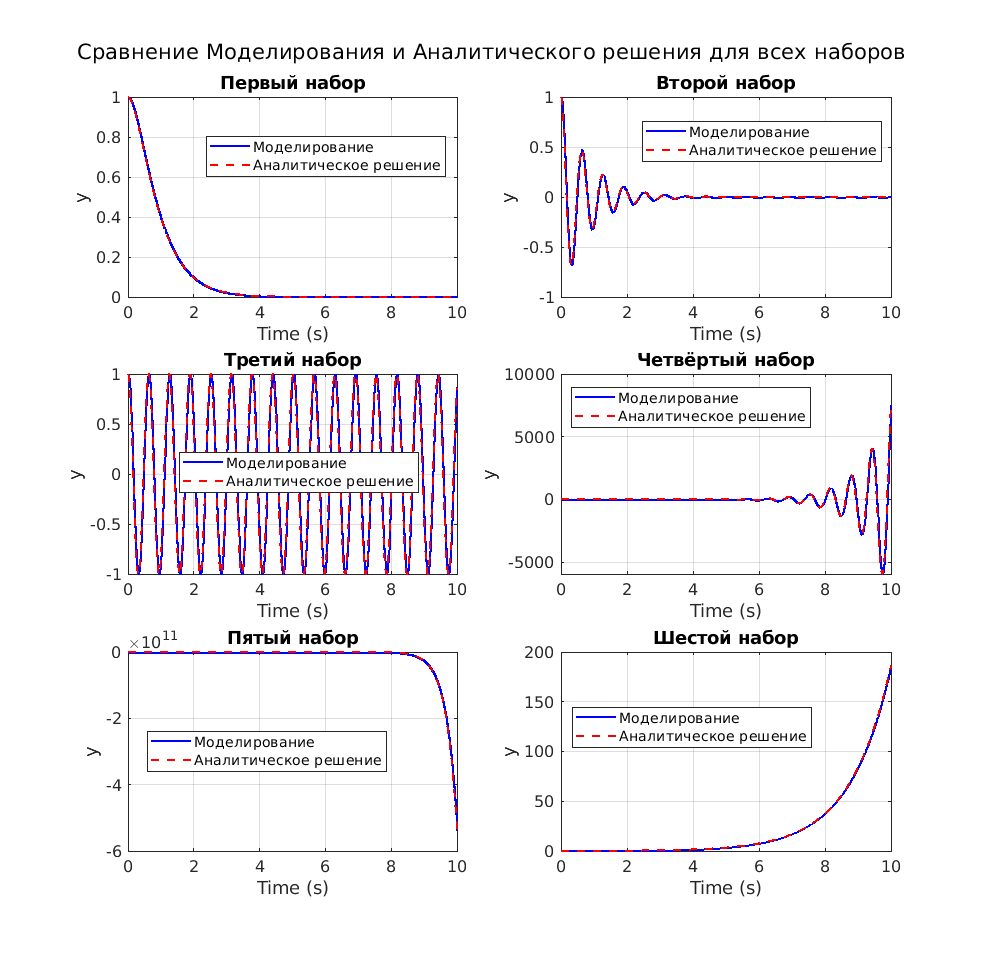
\includegraphics[width=1\textwidth]{figs/task_1_out.png}
    \caption{Графики свободного движения задания 1.}
    \label{fig:task_1_out}
\end{figure}


\section{Область устойчивости}

Рассмотрим систему 3-го порядка, заданную структурной схемой, представленной
на рисунке \ref{fig:task_2_slx}. При значениях постоянных 
времени $T_1=\frac{1}{3}$ и $T_2=\frac{2}{3}$ полюса соответствующих передаточных функций совпадут 
с первым набором корней $\lambda_1=-3$, $\lambda_2=-1.5$ из задания 1.

Определим аналитически границу устойчивости в пространстве параметров $K$ и $T_1$ ($T_2$)
для системы с фиксированным значением T2 ($T_1$) (рассчитанным ранее), 
опираясь на критерий Гурвица. Исходя из структурной схемы, передаточная функция от 
$g$ до $y$ выглядит так
\begin{equation*}
    W=\frac{\dots}{T_1T_2p^3+(T_1+T_2)p^2+p+K},
\end{equation*}
нам нужны только полюса, поэтому числитель не посчитан. Составим матрицу из критерия
Гурвица:
\begin{equation*}
    \begin{bmatrix}
        a_2&a_0&0\\a_3&a_1&0\\0&a_2&a_0
    \end{bmatrix},
\end{equation*}
и откуда получаем условия устойчивости:
\begin{equation*}
    \begin{cases}
        a_2>0,\\
        a_2a_1-a_0a_3>0,\\
        a_0(a_2a_1-a_0a_3)>0,
    \end{cases}\rightarrow
    \begin{cases}
        T_1+T_2>0,\\
        T_1+T_2>KT_1T_2,\\
        K>0.
    \end{cases}
\end{equation*}
Тогда 
\begin{equation*}
    0<K<\frac{T_1+T_2}{T_1T_2},\quad T_1\neq 0, \quad T_2\neq 0,
\end{equation*}
\begin{equation*}
    \text{$K$ - любое если или $T_1=0,\: T_2>0$, или $T_1>0,\: T_2=0$}.
\end{equation*}

Графическое изображение области устойчивости на плоскости
двух параметров $K(T_1)$ и $K(T_2)$ можно увидеть на рисунке \ref{fig:task_2_out}.

Зададимся тремя наборами параметров $K$, $T_1$, $T_2$
\begin{enumerate}
    \item ($2$; $1/3$; $1/10$) - асимптотически устойчивая система,
    \item ($4$; $1/3$; $1$) - система на границе устойчивости,
    \item ($10$; $1/3$; $1$) - неустойчивая система.
\end{enumerate}
Соответствующие симуляции можно видеть на рисунке \ref{fig:task_2_out_1}. Все
в предельно ожидаемо.

\begin{figure}
    \centering
    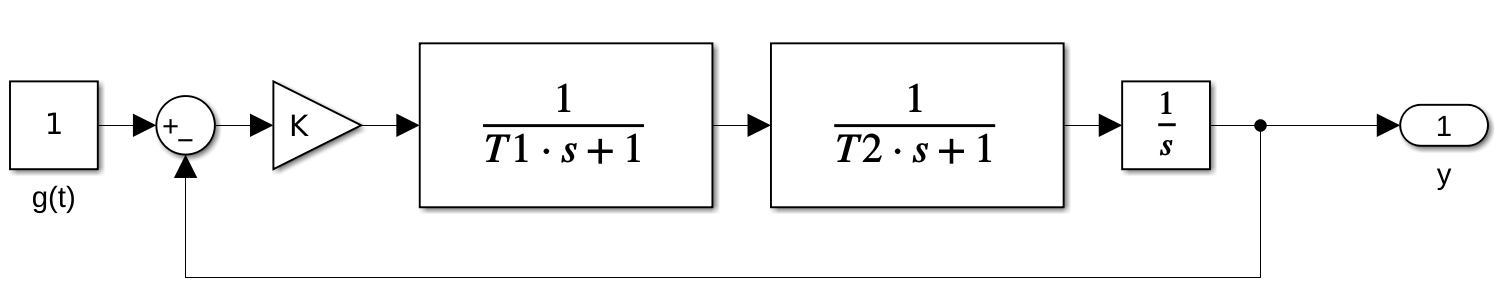
\includegraphics[width=1\textwidth]{figs/task_2_slx.png}
    \caption{Структурная схема системы 3-го порядка задания 2.}
    \label{fig:task_2_slx}
\end{figure}

\begin{figure}
    \centering
    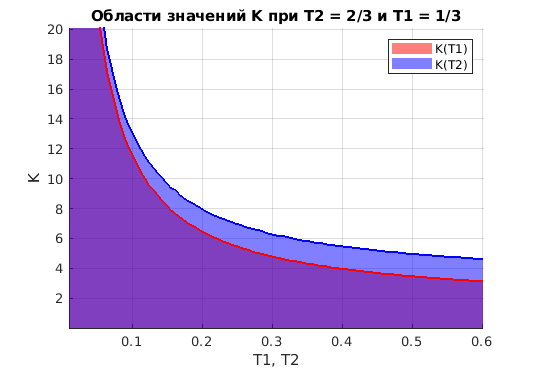
\includegraphics[width=0.8\textwidth]{figs/task_2_out.png}
    \caption{График области устойчивости дифференциального уравнения задания 2.}
    \label{fig:task_2_out}
\end{figure}

\begin{figure}
    \centering
    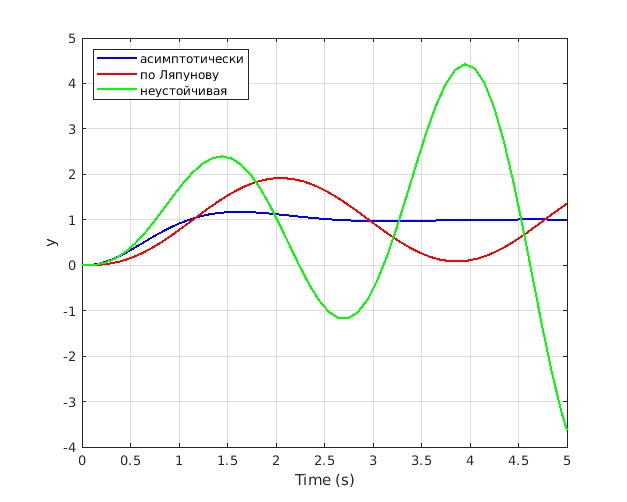
\includegraphics[width=0.8\textwidth]{figs/task_2_out_1.png}
    \caption{График симулирования задания 2.}
    \label{fig:task_2_out_1}
\end{figure}



\section{Автономный генератор}

Для аналитически заданного сигнала $g_{des}(t)=\sin (-3t) + e^{-9t} + e^{-t}$.
в системе вида
\begin{equation*}
    \begin{cases}
        \dot x=Ax,\\
        g=Cx,
    \end{cases},\quad x(0),
\end{equation*}
найдем матрицы $A$ и $C$, и начальные условия. Исходя из желаемого сигнала,
передоточная функция системы имеет такой спектр: \{$-1;\: -9;\: \pm3i$\},
что дает нам построить матрицу
\begin{equation*}
    A=\begin{bmatrix}
        -1&0&0&0\\0&-9&0&0\\0&0&0&3\\0&0&-3&0
    \end{bmatrix},
\end{equation*}
тогда
\begin{equation*}
    e^{At}x(0)=\begin{bmatrix}
        e^{-t}&0&0&0\\0&e^{-9t}&0&0\\0&0&\cos 3t&\sin 3t\\0&0&-\sin 3t&\cos 3t
    \end{bmatrix}
    \begin{bmatrix}
        a_0\\a_1\\a_2\\a_3
    \end{bmatrix}=
    \begin{bmatrix}
        a_0e^{-t}\\a_1e^{-9t}\\a_2\cos 3t+a_3\sin 3t\\-a_2\sin 3t+a_3\cos 3t
    \end{bmatrix},
\end{equation*}
и наконец
\begin{equation*}
    g=Ce^{At}x(0)=\begin{bmatrix}
        c_0&c_1&c_2&c_3
    \end{bmatrix}\cdot e^{At}x(0)=
    c_0a_0e^{-t}+c_1a_1e^{-9t}+(c_2a_2+c_3a_3)\cos 3t+(c_2a_3-c_3a_2)\sin 3t,
\end{equation*}
если приравнять $g=g_{des}$, то получим условия
\begin{equation*}
    \begin{cases}
        c_0a_0=1,\\
        c_1a_1=1,\\
        c_2a_2+c_3a_3=0,\
        c_2a_3-c_3a_2=-1.
    \end{cases}
\end{equation*}
Пусть $C=[1\; 1\; 1\; 0]$, тогда
\begin{equation*}
    x(0)=\begin{bmatrix}
        1\\1\\0\\-1
    \end{bmatrix}.
\end{equation*}
Симуляцию данной системы ВСВ и аналитический сигнал можно увидеть и сравнить
на рисунке \ref{fig:task_3_out}, сигналы очень похожы, что подтверждает
правильность нахождения матриц $A$, $C$ и начальных условий $x(0)$.

\begin{figure}
    \centering
    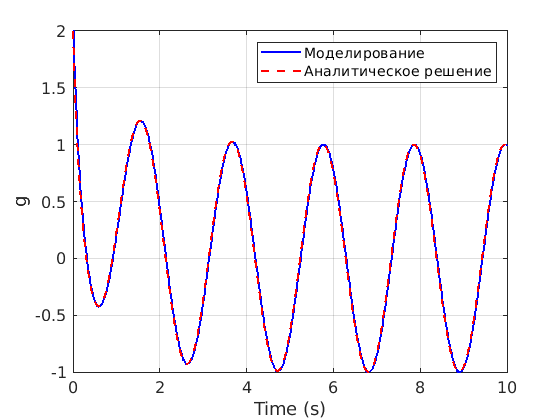
\includegraphics[width=1\textwidth]{figs/task_3_out.png}
    \caption{График симулированной и аналитической функции $g$ задания 3.}
    \label{fig:task_3_out}
\end{figure}




\section{Вывод}

Были рассмотрены различные формы представления линейных динамических
систем: одноканальная В-В, одноканальные канонические управляемая, наблюдаемая,
диагональная В-С-В, многоканальная В-В, многоканальная В-С-В. Для них были составлены
уравнения, построены и симулированы схемы в SIMULINK. По ходу работы как находились
решения систем дифференциальных уравнений, так и решалась обратная задача, зная 
решение найти матрицы и начальные условия системы, что будет полезно
при создании генераторов.


\newpage
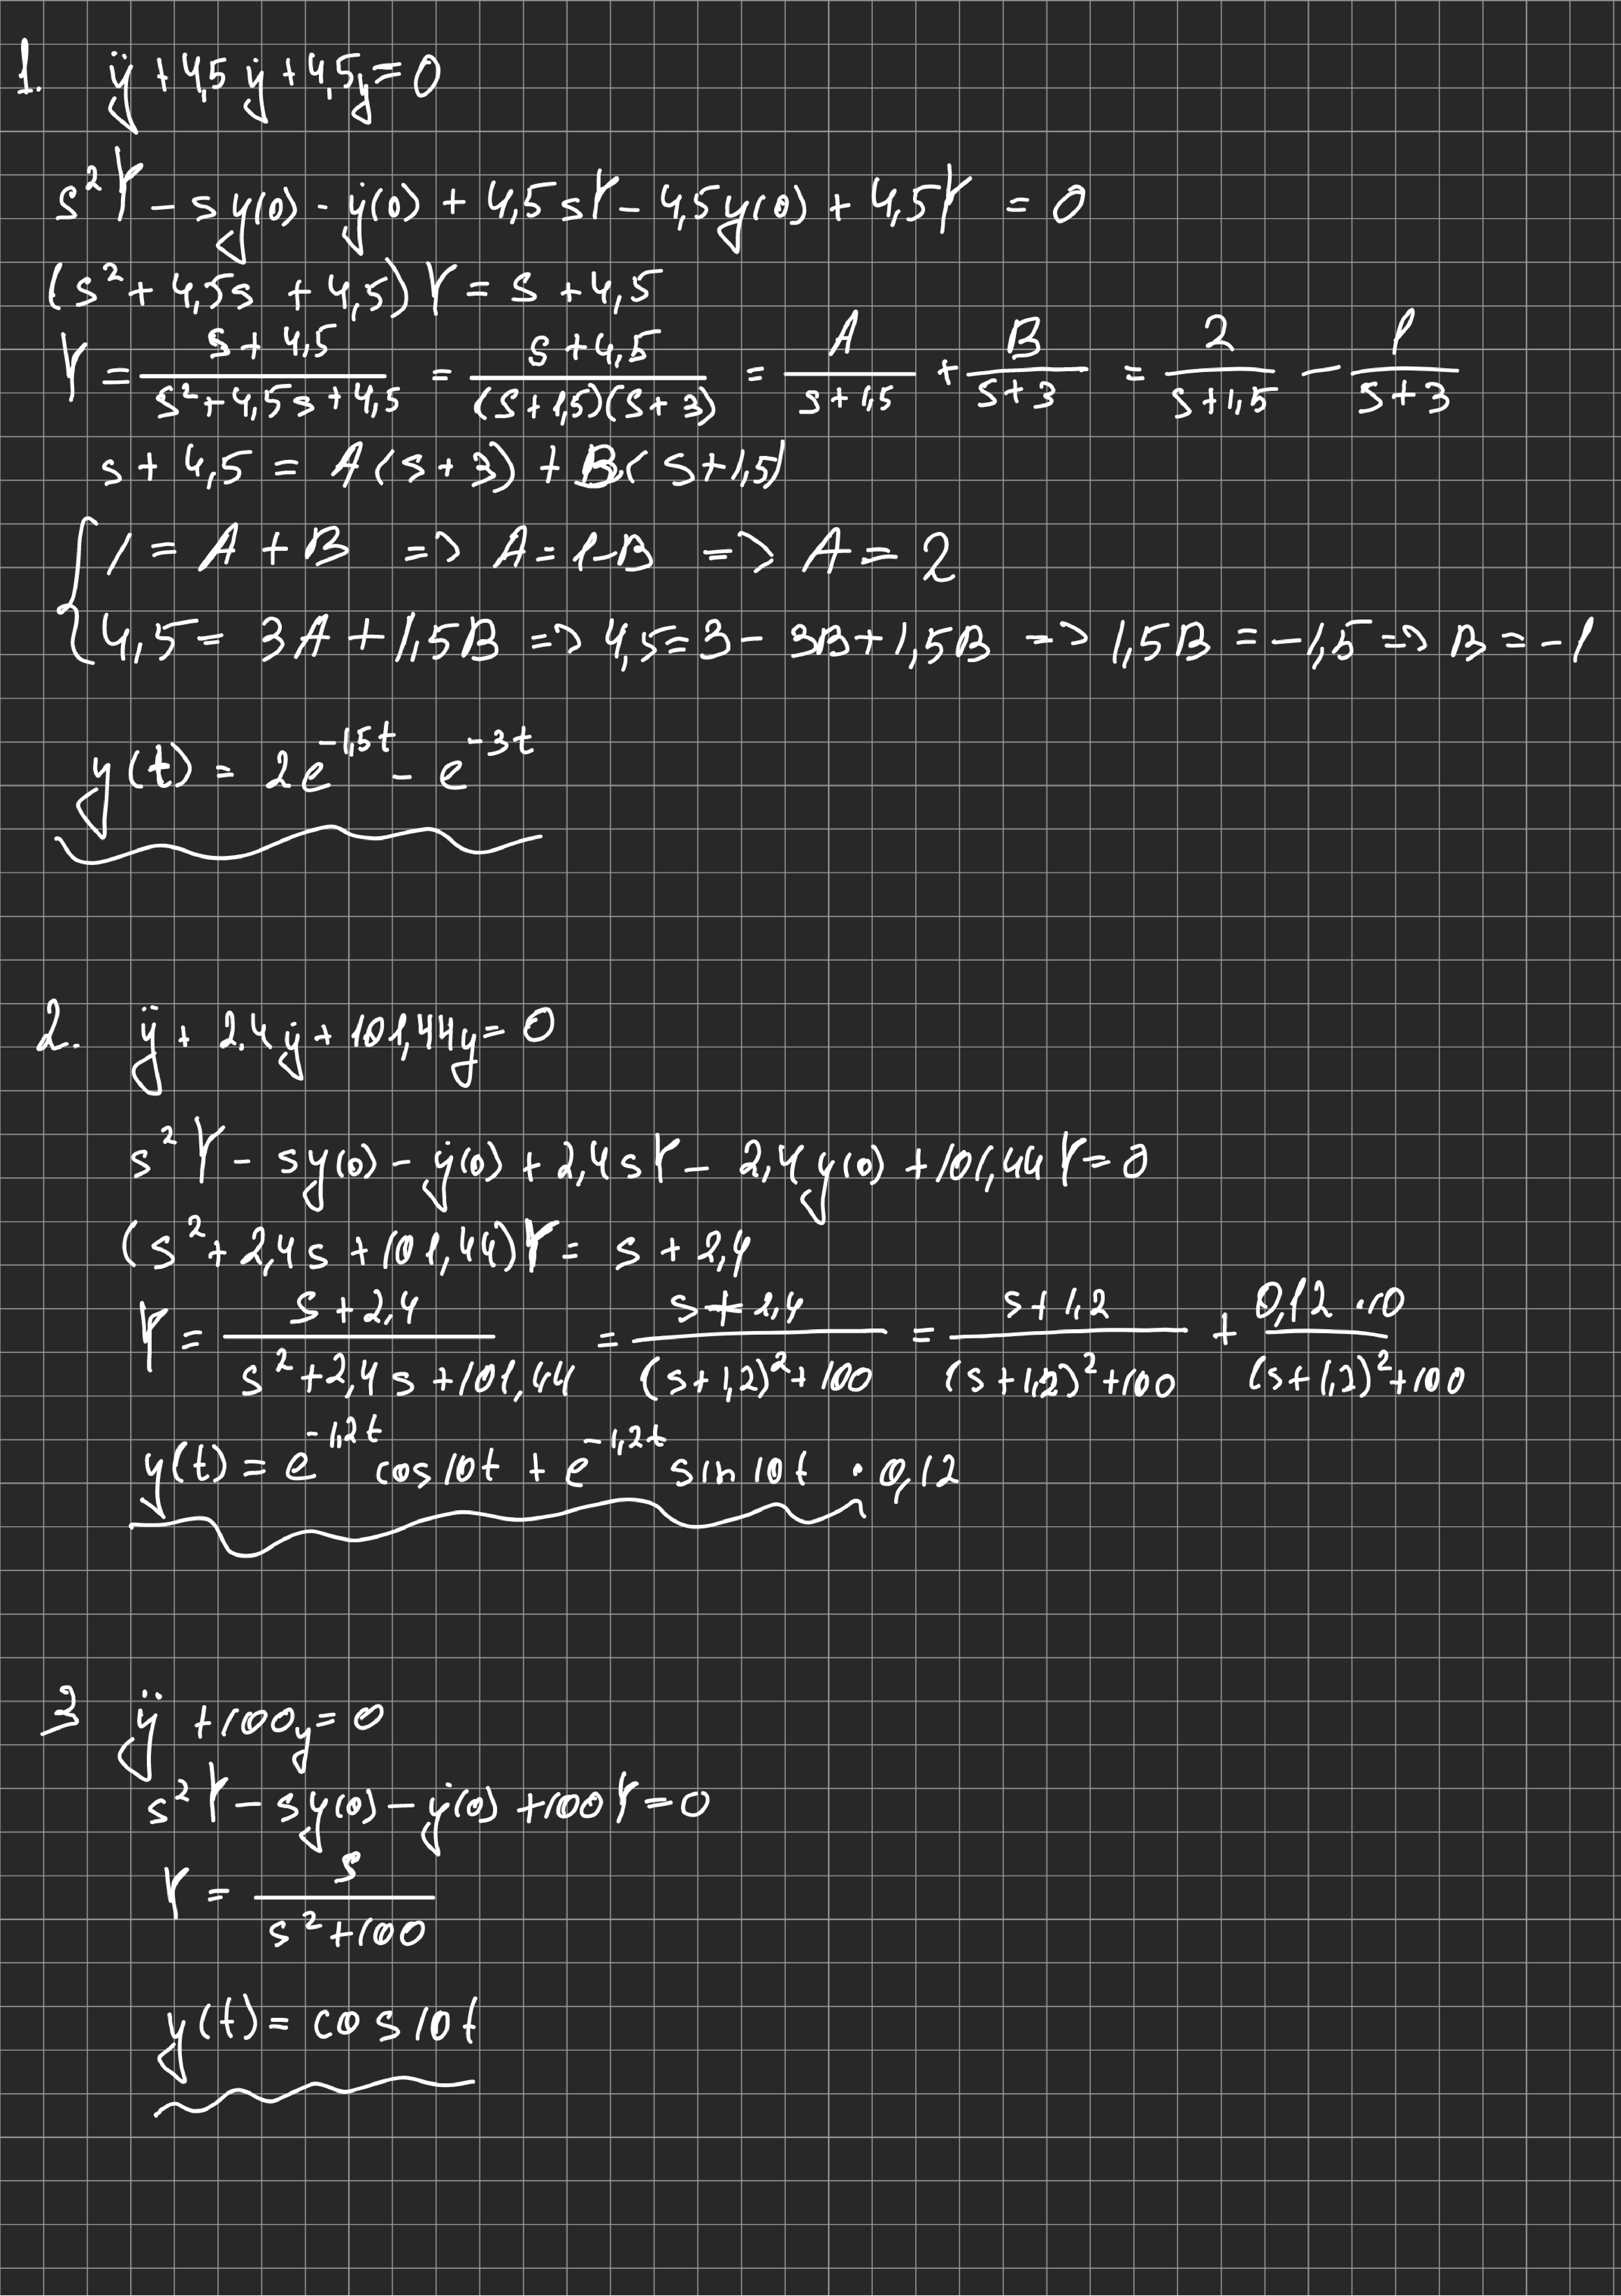
\includepdf[pages=-,scale=1]{figs/analres.pdf}

